\documentclass[spanish,twocolumn]{article}
\usepackage{spconf,amsmath,graphicx}
\usepackage{mathptmx}
\usepackage{mathtools}
\usepackage{amsmath}
\usepackage{mathrsfs}
\usepackage{amssymb}
\usepackage{amsfonts}
\usepackage[utf8]{inputenc}
\usepackage{babel}
\usepackage{color}
\usepackage[Algoritmo]{algorithm}
\usepackage{algpseudocode}
\usepackage{multicol}
\usepackage{caption,setspace}
\usepackage{subfig}
\usepackage{graphicx}

\algrenewcommand\algorithmicif{\textbf{si}}
\algrenewcommand\algorithmicend{\textbf{fin}}
\algrenewcommand\algorithmicfor{\textbf{para}}
\algrenewcommand\algorithmicdo{\textbf{hacer}}
\algrenewcommand\algorithmicwhile{\textbf{mientras}}
\algrenewcommand{\algorithmicrequire}{\textbf{Entrada:}}
\algrenewcommand{\algorithmicensure}{\textbf{Salida:}}
\selectlanguage{spanish}

\def\x{{\mathbf x}}
\def\L{{\cal L}}

\title{OPTIMIZACIÓN MULTIOBJETIVO (FALTA CREAR TITULO) }

\name{Monserrat Mora, Adriana Coronel, Diego Pinto-Roa, José Luis Vázquez Noguera}
\address{Facultad Politécnica - Universidad Nacional de Asunción}

\begin{document}
%	
\maketitle
%
\begin{abstract}

% acá va a ir en unas 2 líneas el problema que se plantea
% la mejora del contraste está relacionada con las métricas que se utilizan para medir la cantidad de información y la calidad de la imagen.
% es necesario que las métricas sean contradictorias para resolver el problema 
% se propone un enfoque de comparación basado en la correlación de pearson para medir la relación inversa entre métricas.
% Los resultados muestran que una dupla de métricas obtiene el coeficiente más bajo de correlación, lo que indica que son los objetivos más contradictorios.

La mejora de contraste en imágenes en escala de gris es una técnica que busca resaltar la información útil de la imagen. Las técnicas, por lo general están relacionadas con las métricas que se utilizan para medir la cantidad de información y la calidad de la imagen. Escoger las métricas adecuadas de forma a lograr maximizar la información disponible minimizando la cantidad de ruido introducido supone un paso fundamental para lograr resultados en el proceso. En este trabajo se propone un enfoque de comparación basado en la Correlación de Pearson para medir la proporción de cambio inversa entre métricas.Los resultados muestran que una dupla de métricas obtiene el coeficiente más bajo de correlación, lo que indica que los objetivos muestran mayor correlación inversa y por lo tanto son las mejores métricas para utilizar dentro del algoritmo de mejora de contraste. Se realizaron comparaciones de a pares entre Entropía, Entropía Local, Índice de Similitud Estructural y la métrica Local Tuned Global.

%Los objetivos propuestos son maximizar la cantidad de información disponible (Entropía / Entropía local) y minimizar la distorsión en las imágenes resultantes (por medio del Índice de Similitud Estructural y el modelo Local Tuned Global) de manera simultánea.

\end{abstract}
%
\begin{keywords}
SMPSO, CLAHE, Entropía, Entropía Local, SSIM, LTG, Mejora del Contraste, Optimización.
\end{keywords}
%
\section{Introducción}
\label{sec:intro}
Las imágenes digitales están expuestas a sufrir una variedad de distorsiones durante su procesamiento, compresión, almacenamiento, transmisión y reproducción, y cualquiera de ellas puede resultar en la degradación de la calidad visual \cite{digitalimganalysis}.

%citaciones sobre algunas de las técnicas existentes. Inclusive sería bueno especificar técnicas basadas en optimización%

El objetivo principal de las técnicas de mejora es procesar una imagen de forma que resulte más adecuada que la original para una aplicación específica. 
En \cite{toolperceptualquality} se propone una evaluación de la calidad perceptible de imágenes monocromáticas, y se realiza una comparación con modelos de calidad basado en la información estructural de la imagen (SSIM) y distribución de Wigner, concluyendo que se debe buscar nuevas métricas que aprovechen las propiedades de los modelos de calidad incluyendo modelos del SVH (Sistema Visual Humano).
En \cite{ssimparametersandwindowsiz} se propone un análisis empírico de los valores más apropiados para las diferentes constantes usadas en las ecuaciones SSIM y la importancia del tamaño de ventana en el cálculo de MSSIM, donde se observó que el comportamiento del SSIM depende de los valores asignados a las constantes y en el tamaño de las ventanas seleccionadas.
En \cite{ltg2014} se propone un modelo que se aproxima al ideal de las métricas de evaluación de la calidad de la imagen(Image quality assesment - IQA), partiendo de la hipótesis de que la percepción de la calidad de la imagen dependen de las distorsiones locales sobresalientes y la degradación de la calidad global, dicho modelo fue comparado con los enfoques clásicos de full-reference (FR) y se concluyó que el modelo propuesto presentaba mejores resultados en comparación a los demás métodos.
Aunque el campo de procesamiento digital de imágenes está construido sobre una base de formulaciones matemáticas y probabilísticas, la intuición y el análisis humano juegan un papel central en la elección de una técnica frente a otra, y esta elección se hace a menudo sobre la base de juicios subjetivos, visuales, por lo tanto, se necesita conseguir medidas cuantitativas que puedan valorar de forma automática la calidad de la imagen percibida.
El histograma de una imagen es ampliamente utilizado como herramienta tanto cualitativa como cuantitativa, es una buena herramienta para la mejora de contraste. Existen enfoques de mejora global y local, los enfoques de mejora local demuestran ser sumamente útiles al momento de realizar detalles en imágenes médicas, y existen diversas propuestas que se centran en mejorar el contraste en radiografías \cite{1625082,4712472,5360176}. Debido a ello en esta  propuesta se analizan pares de métricas de calidad, realizando una comparación de la correlación entre las mismas, la entropía/entropía local vs. SSIM y entropía/entropía local vs LTG, para identificar las métricas más adecuadas para la optimización multiobjetivo de la mejora de contraste de una imagen. 
Se utilizará una meta heurística de optimización de objetivos, de manera a sintonizar los parámetros de entrada del algoritmo de mejora del contraste descripto en la sección \ref{sec:clahe}, de manera a obtener un grupo de imágenes contrastadas, las cuales serán evaluadas en cuanto a la ganancia de información proveída y distorsión introducida por la ecualización (sección \ref{sec:metricas}).
El resto del trabajo se organiza de la siguiente manera: En la sección \ref{sec:clahe} se describe brevemente el algoritmo de mejora de contraste adoptado; en la sección \ref{sec:metricas} se muestran las métricas de evaluación de resultados utilizadas; en la sección \ref{sec:formulacion} se plantea de manera formal el problema que se intenta resolver; en la sección \ref{sec:propuesta} se muestra la aplicación de la correlación entre las métricas seleccionas %no estoy segura que poner aca%; luego en la sección \ref{sec:resultadosdiscusion} se discuten los resultados, y finalmente en la sección \ref{sec:conclusion} se detallan las conclusiones correspondientes.



%lo que considero fundamental es que se distinga ya en la introducción, que este trabajo trata sobre el problema de selección de métricas para la optimización multiobjetivo de la mejora de contraste, y no sobre la optimización en sí%

\section{Contrast Limited Adaptive Histogram Equalization (CLAHE)}
\label{sec:clahe}
Este enfoque de mejora de contraste presentado en \cite{Zuiderveld:1994:CLA:180895.180940} es una extensión del algoritmo original Adaptive Histogram Equalization (AHE) \cite{pizer1987adaptive}; en ambos métodos se implementa un enfoque de Ecualización del Histogama local basada en {\it Regiones Contextuales}, que representan porciones de la imagen, cuyas dimensiones están delimitadas por $(\mathcal{R}_x, \mathcal{R}_y)$, para realizar la ecualización por sectores de la imagen. Las inconsistencias entre fronteras de las secciones la imagen se corrigen aplicando un esquema de interpolación bilineal. 
El algoritmo AHE original presenta problemas de amplificación del ruido, por tanto en CLAHE se implementa una limitación de la cantidad de pixeles que pueden alcanzar cierto nivel de gris dentro del histograma local; aquí se define el coeficiente {\it Clip Limit} $\mathcal{C}$, como un factor que está fuertemente relacionado con los contenidos del histograma. El mismo permite realizar cortes en picos del histograma local, que se traducen en ruido dentro de la imagen.

%acá hay algo importante que creo que falta, hay que mostrar que clahe (y sus posibles variantes) son muy efectivas para realizar la mejora del contraste en imágenes médicas; además podemos agregar alguna grafiquita, porque de otra forma queda muy escueto%

\section{métricas de evaluación}
\label{sec:metricas}
Se realiza una selección de alternativas a partir de la necesidad de encontrar métricas que proporcionen el mejor balance entre mejora del contraste y distorsión. En esta sección se muestran las cuatro métricas seleccionadas para el análisis y comparaciones de correlación entre las mismas. Éstas son la Entropía y Entropía local como medidas de mejora del contraste, el Índice de Similitud Estructural y el modelo Local Tuned Global como medidas de distorsión de la imagen.

\subsection{Entropía}
\label{ssec:entropia}

La {\it Entropía de la Información} es una medida de la aleatoriedad presente en la imagen \cite{tsai2008information}, en donde valores altos indican imágenes ricas en detalles, y por tanto poseen alto contraste. Se puede definir la Entropía de la imagen como: 

\begin{equation}\label{eq:entropia}
\mathscr{H}=-\sum_{i=0}^{L-1}\mathcal{P}_i log_2(\mathcal{P}_i) [bits] \quad \mathscr{H} \in {0,..,log_2(L)} 
\end{equation}

Donde $\mathcal{P}_i$ es la probabilidad de ocurrencias del nivel de gris $i$ en el histograma y $L$ es el máximo nivel de gris que se puede utilizar para representar la imagen. Esta métrica es interesante debido a que está fuertemente asociada al brillo medio de la imagen \cite{108593}; este coeficiente nos ayuda a ver cuánto aumenta el contraste como consecuencia de la transformación de la imagen.


\subsection{Entropía Local}
\label{ssec:entropialocal}


\subsection{Índice de similitud estructural (SSIM)}
\label{ssec:ssim}
El {Índice de Similitud Estructural (SSIM)} \cite{wang2004image} es un coeficiente que mide el grado de distorsión producida en una imagen resultante $T$ a consecuencia de aplicar una Mejora del Contraste a una imagen original $I$. 
EL SSIM mide las similitudes entre tres elementos de las dos imágenes: la luminancia (intensidad media), el contraste y la estructura. SSIM se calcula por bloques, por lo que si definimos dos ventanas $I_x$ e $T_y$ para las imágenes original y resultante, respectivamente, se define el SSIM como se muestra abajo:

\begin{equation}\label{eq:ssim}
\resizebox{.9\hsize}{!}
{
$SSIM(I,T)=\frac{(2\mu_{I_x}\mu_{T_y}+C_1)(2\sigma_{I_xT_y}+C_2)}{(\mu_{I_x}^2+\mu_{T_y}^2+C_1)(\sigma_{I_x}^2+\sigma_{T_y}^2+C_2)} \quad SSIM \in [0,1]$
}
\end{equation}

Donde $\mu_{I_x}$ es el promedio de intensidades de $I_x$; $\mu_{T_y}$ es el promedio de intensidades de $T_y$; $\sigma_{I_x}^2$ y $\sigma_{T_y}^2$ son las varianzas de intensidades de $I_x$ e $T_y$, respectivamente; $\sigma_{I_x T_y}$ es la covarianza entre $I_x$ e $T_y$; $C_1=(K_1L^2)$, $L$ es el rango dinámico de intensidades de los pixeles (256 para una imagen en escala de grises de 8 bits) y $K_1 \ll 1$ es una constante pequeña; $C_2=(K_2 L)^2$, y $K_2 \ll 1$; tanto $C_1$ y $C_2$ son constantes que se usan para estabilizar la division en caso de que el denominador tienda a cero.

\subsection{ Local Tuned Global Model (LTG)}
\label{ssec:ltg}
El modelo {Local Tuned Global (LTG)} está inspirado en las métricas IQA (Image Quality Assessment)\cite{ltg2014}, fue introducido bajo la hipótesis de que la percepción visual humana en  la calidad de la imagen depende de la distorsión local resaltante y la degradación global de la calidad. 
El LTG es un enfoque basado en el gradiente de la imagen, ya que ésta es muy sensible a las distorsiones de la misma; así también extrae información sobre la luminancia (brillo percibido por el ojo humano) y la crominancia (información del color) de la imagen de entrada y la imagen distorsionada, luego mide la distorsión local resaltante y la degradación global de la calidad en la información obtenida sobre la luminancia y compara las diferencias en la información obtenida sobre la crominancia, derivando así el valor global de la calidad de la imagen.

\begin{equation}\label{eq:ltg}
\resizebox{.6\hsize}{!}
{
$LTG(x,y) =\frac{\Phi(G_{s}^{\theta_1})}{\Phi(G_{m}^{\theta_2})} \Phi(I_{m}^{\theta_3}.Q_{m}^{\theta_3})$
}
\end{equation}

El GM está dada por:
\begin{equation}\label{eq:gm}
\resizebox{.4\hsize}{!}
{
$G = \sqrt[]{G_{h}^{2} + G_{v}^{2}}$
}
\end{equation}

Donde:
\begin{itemize}
 \item $G_{m}$ =  es el gradiente medio de la imagen original y distorsionada, se adopta el operador Scharr  \cite{gradiente}.
 \item $ G_{s}$ = indica los pixeles con valores S\% más altos en $G_{m}$.
 \item  $I_{m}$ y $Q_{m}$ = contienen la información de crominancia de las imagenes. 
\end{itemize} 

%Ésto vamos a poner en una sección aparte, hay que hacer hincapié en que el problema que se resuelve es la selección de métricas, y ésta es la herramienta que se usa para medir qué tan contradictorias son las métricas%
\subsection{Correlación de Pearson}
\label{ssec:correlacion}
Es un índice que puede utilizarse para medir el grado de relación o covariación de dos variables distintas relacionadas linealmente,  siempre y cuando ambas sean cuantitativas.

El valor del  índice de correlación varía en el intervalo [-1,1]. Esto es, si tenemos dos variables $X$ e $Y$, y definimos el coeficiente de correlación de Pearson entre estas dos variables como $r_{xy}$ entonces: 
\begin{equation}\label{eq:gm}
\resizebox{.3\hsize}{!}
{
$-1<r_{xy}<1$ 
}
\end{equation}

Donde:
\begin{itemize}
\item Si $r = 1$, existe una correlación positiva perfecta. Significa que existe relación directa entre las dos variables, cuando una de ellas aumenta, la otra también lo hace en proporción constante.
\item Si $0<r<1$, existe una correlación positiva.
\item Si $r = 0$, no existe relación lineal.
\item Si $-1<r<0$, existe una correlación negativa.
\item Si $r = -1$, existe una correlación negativa perfecta. El índice indica que existe una relación inversa entre las dos variables: cuando una de ellas aumenta, la otra disminuye en proporción constante.
\end{itemize}

\section{Formulación del Problema Planteado}
\label{sec:formulacion}
%el problema planteado vamos a tener que revisarlo, porque en este caso no es directamente la aplicación del la metaheurística para la mejora del constraste, sino que es la evaluación de las métricas que dan menor correlación%
Dadas la imagen de entrada $I$, y un vector $\overrightarrow{x}=(\mathcal{R}_x, \mathcal{R}_y, \mathcal{C})$, donde $\mathcal{R}_x$ y $\mathcal{R}_y$ conforman la región contextual y $\mathscr{C}$ es el $Clip Limit$, se desea calcular el conjunto de soluciones $\mathscr{X}$ que maximice de manera simultánea los objetivos $f_1$ y $f_2$, como se muestra abajo:

\begin{equation}\label{eq:fitness}
    f(I, \overrightarrow{x}) = \{ f_1(I, \overrightarrow{x}), f_2(I, \overrightarrow{x}) \} \qquad f_1,f_2 \in [0,1]
\end{equation}

donde:
\begin{itemize}
%\item $\overrightarrow{x}=(\mathcal{R}_x, \mathcal{R}_y, \mathcal{C})$, donde $\mathcal{R}_x$ y $\mathcal{R}_y$ conforman la región contextual y $\mathscr{C}$ es el Clip Limit.
\item $f_{1}(I, \overrightarrow{x})=\frac{\mathscr{H}(T)}{log_{2}L}$ es la Entropía local normalizada de la imagen $T$.
\item $f_{2}(I, \overrightarrow{x})=SSIM(I,T)$ es el Índice de Similitud Estructural o  el modelo Local Tuned Global  entre $I$ y $T$.

Siendo $T$ la imagen mejorada por $CLAHE(\overrightarrow{x},I)$ con los parámetros dados por $\overrightarrow{x}$ aplicados a $I$.

\end{itemize}

sujeto a:

\begin{itemize}
\item $\mathcal{R}_x \in [2,..,M]$ en los números $\mathbb{N}$.
\item $\mathcal{R}_y \in [2,..,N]$ en los números $\mathbb{N}$.
\item $\mathscr{C} \in (0,1]$ en los números $\mathbb{R}$.
\end{itemize}

Ésto significa que los valores de $\mathcal{R}$ solamente pueden tomar valores enteros positivos entre $(2,2)$ y $(M,N)$ y que $\mathscr{C}$ puede tomar un valor mayor a cero y menor o igual a 1.



\section{propuesta}
\label{sec:propuesta}
%aca la propuesta no es aplicar directamente el algoritmo, hay que acortar un poquito la parte del smpso, e incluir como marco teorico. Despues vamos a desarrollar la propuesta en si.
Se utiliza el algoritmo $SMPSO$ \cite{4938830}, donde las soluciones potenciales $\overrightarrow{x}=(\mathcal{R}_x, \mathcal{R}_y, \mathcal{C})$ se denominan {\it partículas} y el conjunto de partículas $\Omega$ se denomina {\it enjambre}. Cada partícula $\overrightarrow{x_i}$ se actualiza en cada generación $t$ de acuerdo a la siguiente ecuación:

\begin{equation}\label{eq:psobasico}
\overrightarrow{x_i}^t = \overrightarrow{x_i}^{(t-1)} + \overrightarrow{v_i}^t
\end{equation}

donde el factor $\overrightarrow{v_i}$ se conoce como la velocidad y está dado por:

\begin{equation}\label{eq:psobasico2}
\overrightarrow{v_i}^t = \omega \cdot \overrightarrow{v_i}^{(t-1)} + C_1 \cdot r_1 \cdot (\overrightarrow{x_{p_i}}-\overrightarrow{x_i}) + C_2 \cdot r_2 \cdot (\overrightarrow{x_{g_i}}-\overrightarrow{x_i})
\end{equation}

Aquí, $\overrightarrow{x_{p_i}}$ es la mejor solución que encontró $\overrightarrow{x_i}$, $\overrightarrow{x_{g_i}}$ es la mejor partícula (también conocida como {{\it líder}) que se encuentra en todo el enjambre, $\omega$ es el peso de la inercia de la partícula, $r_1$ y $r_2$ son dos números aleatorios, y $C_1$ y $C_2$ son parámetros que controlan el efecto de las partículas locales  y globales. Si una partícula es mejor que otra, se dice que la $domina$, y la dominancia está definida de la siguiente manera: $\overrightarrow{x_{g_i}} \succ \overrightarrow{x_i}$ si y sólo si

\begin{equation}\label{eq:dominanciapareto}
         \begin{cases}  f_i(I,\overrightarrow{x_{g}})  \geq f_i(I,\overrightarrow{x}) \forall i \in \{1,2\} \\
                        f_i(I,\overrightarrow{x_{g}}) > f_i(I,\overrightarrow{x}) \exists i \in \{1,2\} \\
         \end{cases}
\end{equation}

El {\it Conjunto Pareto} es el grupo de soluciones $\mathscr{X}$, y la imagen en el espacio objetivo es el {\it Frente Pareto}.

En adición, en $SMPSO$ se realiza una restricción en $\overrightarrow{v}$, para cada componente $j$ de $\overrightarrow{x}$, de acuerdo a la siguiente ecuación: 
                
\begin{equation}\label{eq:restricciondelta}
    v_{i,j}^t = \begin{cases}  delta_j &\mbox{if } v_{i,j}^t > delta_j \\
                                -delta_j & \mbox{if } -delta_j \\
                                v_{i,j}^t & otherwise \end{cases}
\end{equation}

donde: 
\begin{equation} \label{eq:restricciondelta2}
delta_j= \frac{upper\_limit_j - lower\_limit_j}{2}
\end{equation}

El \textbf{Algoritmo \ref{alg:pso_clahe}} muestra cómo se implementa la propuesta. Las imágenes resultantes se evalúan de acuerdo a las métricas \eqref{eq:entropia} y \eqref{eq:ssim} o \eqref{eq:ltg}, y los mejores resultados que se obtienen en base a éstas métricas conforman un conjunto pareto de soluciones. El conjunto representa una serie de imágenes con distintos niveles de contraste, de manera a resaltar características particulares de la misma.

La interacción entre CLAHE y las partículas de SMPSO se muestran en la \textbf {Fig. 1}. CLAHE recibe como parámetros de entrada los valores almacenados por una partícula $(\mathcal{R}_x,\mathcal{R}_y, \mathscr{C})$ y la imagen original $I$, y a la imagen procesada se le calculan las métricas $\mathscr{H}$ y $SSIM$  o $LTG$ de manera a obtener las funciones objetivo. Las soluciones no dominadas se almacenan en el conjunto pareto. Éste proceso se repite hasta alcanzar un criterio de parada definido.

% \begin{minipage}[b]{1.0\linewidth}
%   \vspace{0.5cm}
%   \centering
%   \centerline{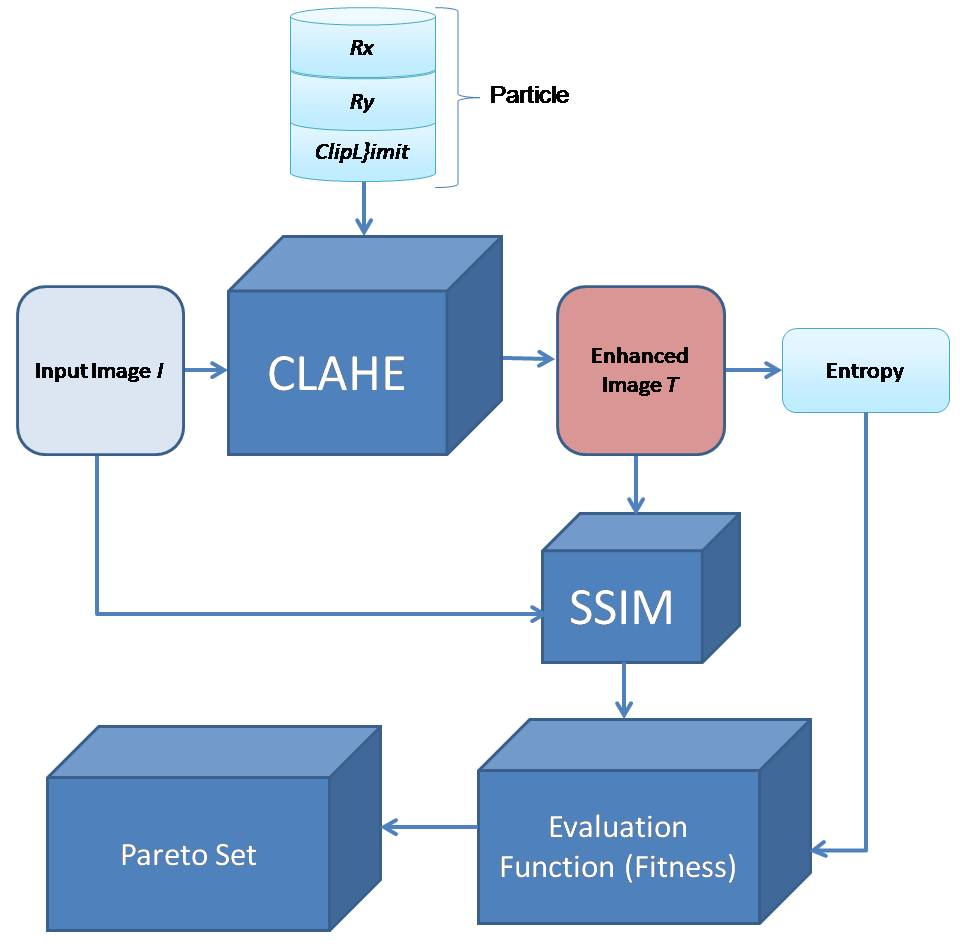
\includegraphics[height=6.5cm]{Figures/particula_clahe2.png}}
%   \vspace{0.5cm}
%   \label{fig:particula_clahe}
%   \captionof{figure}{Interacción entre CLAHE y SMPSO.}
% \end{minipage}

 \twocolumn
 \bibliographystyle{IEEEbib}
 \bibliography{refs1}



\end{document}
